\documentclass[11pt]{article}
%\renewcommand{\thesection}{\Roman{section}}  %zmiana section na rzymskie
\usepackage{amsmath, amsfonts, amsthm, amssymb}   % matematyka
\usepackage[utf8]{inputenc}
\usepackage{polski}
\usepackage[margin=60pt]{geometry}
%\usepackage[usenames,dvipsnames,table,xcdraw]{xcolor} % kolorowanie 
\usepackage{array} % taka tabelka dobra do macierzy
\usepackage{multirow}
\usepackage{hyperref} % linkowanie
\usepackage{relsize}
\usepackage{graphicx} 
\usepackage{color}
%%%%%%%%%%%%%%%%%%%%%%%%%%%%%%%%%%%%%%%%%%%%%%%%%%%%%%%%%%%%%%%%%%%%%%%%%%%%%%%%%%
% 
%%%%%%%%%%%%%%%%%%%%%%%%%%%%%%%%%%%%%%%%%%%%%%%%%%%%%%%%%%%%%%%%%%%%%%%%%%%%%%%%%%

%\newcommand{\ul}[1]{\ensuremath{\underline{#1}}}
\renewcommand{\r}{\vec{r}}
\renewcommand{\j}{\vec{j}}
\renewcommand{\v}{\vec{v}}
\newcommand{\B}{\vec{B}(\vec{r},t)}
\newcommand{\E}{\vec{E}(\vec{r},t)}
\renewcommand{\arg}{(\vec{r},t)}
\newcommand{\argg}{(\vec{r},\vec{r}',t,t')}
\newcommand{\ave}[1]{\left< #1 \right>}
\newcommand{\Brho}{\mathlarger{\mathlarger{\rho}}}
\newcommand{\p}{\vec{p}}
\newcommand{\dt}{\frac{d}{dt}}
\newcommand{\nab}[1]{\nabla_{\vec{#1}}}
\newcommand{\rpt}{(\vec{r},\vec{p},t)}
\newcommand{\qp}{(\vec{q},\vec{p})}
\newcommand{\qpt}{(\vec{q},\vec{p},t)}
\newcommand{\f}{f\rpt}
\newcommand{\Ep}{E(\p)}
\newcommand{\ka}{\vec{k}}
\newcommand{\fp}{f(\vec{r},\vec{p}~',t)}

\title{Wstęp do kwantowej teorii transportu elektronowego}
\author{Sylwia Gołąb, Paweł Rzońca}

\graphicspath{ {./obrazki/} }

\begin{document}

\maketitle

\tableofcontents
\newpage


%%%%%%%%%%%%%%%%%%%%%%%%%%%%%%%%%%%%%%%%%%%%%%%%%%%%%%%%%%%%%%%%%%%%%%%%%%%%%%%%%%
% the text
%%%%%%%%%%%%%%%%%%%%%%%%%%%%%%%%%%%%%%%%%%%%%%%%%%%%%%%%%%%%%%%%%%%%%%%%%%%%%%%%%%


\section{Początki teorii elektronowej (subiektywnie)}
\begin{table}[h!]
    \centering
    \begin{tabular}{ll|ll|ll}
        \multicolumn{2}{c}{Elektrodynamika} & 
		\multicolumn{2}{|c|}{Teoria kinetyczna} & 
		\multicolumn{2}{c}{Teoria kwantowa} \\
            &&   1803 r. J. Dalton: & atomy   &&     \\
        1822 r. H. Davy: & $\sigma \sim S/L$ &&    &&     \\
        1826 r. G. Ohm: & $I \sim V$         & 1827 r. R. Brown: & ruchy  && \\
        1845 r. G. Kirchhoff: & $ j \sim E_f$& &&& \\
        1861 r. J. Maxwell: & równania & 1860 r. J. Maxwell: & rozkład $v$ && \\
        && 1865 r. J. Loschmidt: & rozmiar at. && \\
        && 1867 r. J. Maxwell: & równanie && \\
        && \multicolumn{2}{r|}{ciągłości o strukturze r. kinet.} && \\
        && 1872 r. L. Boltzmann: & równanie && \\
        1881 r. Helmholtz: & \multirow{2}{*}{elektron} &&&&\\
        Johnstone Stoney: &  &&&& \\
        1897 r. J. J. Thompson && 1900 r. D. Hilbert && 1900 r. M. Planck & \\
	&& 1905 r. Einstein i  & teoria r. && \\
	&& Smoluchowski: & Browna && \\ 
	1908 r. R. Millikan:& wart. $e$ &&&& \\ 
	1910 r. E. Rutherford:& budowa at. &&&&\\
	&& 1913 r. Bohr:& model at. && \\
	1916 r. Tolman-Steward:& bezwł. el. &&&&\\
	&&&& 1924 r. L. de Broglie & \\
	&&&& 1926 r. E. Schr\"{o}dinger & \\
	&&&& 1927 r. Fermi i Dirac: & stat. kw. \\
    \end{tabular}
\end{table}
Elektronowa teoria meterii 
\begin{itemize}
	\item[1845 r.] G. Fechner - Model prądu elektronowego 
	\item[1846 r.] W. Weber - Elektrodynamika cząstek
		$$ F = \dfrac{q_1q_2}{r^2} \left\{ 1 + \dfrac{r}{c^2} \ddot{r} (t) -
		\dfrac{1}{2c^2} \left[ \dot{r} (t) \right]^2 \right\} $$
	\item[1881 r.] Helmholtz
	\item[1897 r.] H. A. Lorentz - teoria elektronowa
	\item[1898 r.] E. Riecke - 
	\item[1900 r.] Drude - model przewodnictwa
	\item[1927 r.] Sommerfeld A. - statystyki kwantowe do opisu elektronów
	\item[1928 r.] Block
\end{itemize}
Teorie na przestrzeni czasu:
\begin{itemize}
	\item[1900 $\div$ 1927] Klasyczna teoria transportu elektronowego 
	\item[1927 $\div$ 1928] Półklasyczna teoria transportu elektronowego
	\item[1928 $\div$ 1933] Współczesna teoria transportu elektronowego 
\end{itemize}

%%%%%%%%%%%%%%%%%%%%%%%%%%%%%%%%%%%%%%%%%%%%%%%%%%%%%%%%%%%%%%%%%%%%%%%%%%%%%%%%%%
% new subsection
%%%%%%%%%%%%%%%%%%%%%%%%%%%%%%%%%%%%%%%%%%%%%%%%%%%%%%%%%%%%%%%%%%%%%%%%%%%%%%%%%%
\section{Teoria elektronowa Lorenza}
\textbf{Założenia:}
\begin{enumerate}
	\item Ośrodki materiale mają strukturę dyskretną, tzn. zbudowane są z 
		cząstek naładowanych, które w sumie dają układ neutralny.
	\item Wszystkie zjawiska w ośrodku materialnym są spowodowane ruchem 
		cząstek naładowanych pod wpływem pól zewnętrznych, przy czym:
		\begin{enumerate}
			\item w dielektrykach cząstki naładowane są związane i mogą
				wykonywać drgania wokół położeń równowagi lub ulegać
				nieznacznym wychyeniom pod wpływem przyłożonego $\vec{E}$,
			\item w przewodnikach prócz cząstek związanych występują także
				czastki naładowane swobodne, których ruch powoduje 
				powstanie prądu elektrycznego,
			\item w ośrodkach magnetycznych istnieją cząstki naładowane 
				posiadające wewnętrzny moment magnetyczny lub niezerowy
				moment pędu.
		\end{enumerate}
	\item Mikroskopowe pola elektromagnetyczne wytwarzane przez cząstki 
		naładowane tworzące rozpatrywany ośrodek są rozwiązaniami 
		równań Maxwella w próżni:\\
	\begin{equation}{\label{Max_mikro}}
	\left\{ 
		\begin{array}{l}
		\nabla \circ \vec{e} (\vec{r},t) = \rho(\vec{r},t)\\
		\nabla \times \vec{b}(\vec{r},t) - \partial_t \vec{e}(\vec{r},t) 
			= \vec{j}(\vec{r},t)\\
		\nabla \times \vec{e} (\vec{r},t) + \partial_t \vec{b} (\vec{r},t)
			= \vec{0} \\
		\nabla \circ \vec{b} (\vec{r},t) = 0.
		\end{array}
	\right.
	\end{equation}
	$\vec{e}(\vec{r},t), \ \vec{b}(\vec{r},t)$  - mikroskopowe pola elektryczne i
		magnetyczne \\
	$\rho (\vec{r},t)= \sum_i q_i \delta (\vec{r} -  \vec{r_i} (t))$\\
	$\vec{j}(\vec{r},t)= \sum_i \vec{v_i} (t) \delta(\vec{r} - \vec{r_i}(t))$
	\item Gęstość siły działająca na $\vec{\rho}(\vec{r},t)$ ma postać
	$$ \vec{f}(\vec{r},t) = \vec{\rho}(\vec{r},t) [ \vec{e}(\vec{r},t)+ \vec{v}(t)
		\times \vec{b}(\vec{r},t)] $$
	$$ \vec{F} (t) = \int d^3r' f(\vec{r}\ ',t) = $$
	przy założeniu jednorodności $\vec{b}$ i $\vec{e}$
	$$ = \int d^3r' \{ \rho \arg [ \vec{e} + \vec{v}(t) \times \vec{b} ]  \} =
	\int d^3r' \{ q \delta (\vec{r} - \vec{r}\ ') [ \vec{e} + \vec{v}(t) 
	\times \vec{b} ] \} = q[ \vec{e} + \vec{v}(t) \times \vec{b} ] \int d^3r' 
	\delta (\vec{r} - \vec{r} \ ').$$
	Ostatecznie
	\begin{equation}
		\vec{F} = q (\vec{e} + \vec{v} \times \vec{b})
	\end{equation}
	\begin{equation}
		m\ddot{\vec{r}} (t) = q[ \vec{e} + \vec{v} (t) \times \vec{b} ]. 
	\end{equation}
\end{enumerate}
Zmiany przestrzenne $\vec{e} \arg$ i $\vec{b} \arg $ są znaczące na odcinkach
rzędu $10^{-10} \mbox{m} = 1 \stackrel{\circ}{\mbox{A}} = 0,1 \mbox{nm}.$\\
Zmiany czasowe są rzędu $10^{-13} \div 10^{-17}$s. 
\\
Klasyczny promień elektronu $r_e = \frac{1}{4\pi \epsilon_0} \frac{e^2}{mc^2} 
\approx 2,82 \cdot 10^{-6}$nm, rozmiar protonu $r_p \approx 0,88 \cdot 
10^{-6}$nm natomiast promień atomu $r_p \approx 0,1$nm.

%%%%%%%%%%%%%%%%%%%%%%%%%%%%%%%%%%%%%%%%%%%%%%%%%%%%%%%%%%%%%%%%%%%%%%%%%%%%%%%%%%
% new section
%%%%%%%%%%%%%%%%%%%%%%%%%%%%%%%%%%%%%%%%%%%%%%%%%%%%%%%%%%%%%%%%%%%%%%%%%%%%%%%%%%
\section{Makroskopowa elektrodynamika ośrodków materialnych}
\textbf{Hipotezia: }
Makroskopowe pola $\vec{E}$ i $\vec{B}$ są wartościami średnimi pól 
mikroskopowych$\vec{e}$ i $\vec{b}$.
\begin{equation}
	\vec{E} \arg = \left< \vec{e} \arg \right>
\end{equation}
\begin{equation}
	\vec{B} \arg = \left< \vec{b} \arg \right>,
\end{equation}
gdzie średnia jest przestrzenna, czyli
$$ \left< \vec{f} \arg \right> \equiv \int d^3 r' w(\vec{r}\ ')\vec{f}
( \vec{r} - \vec{r}\ ',t). $$
$w(\vec{r}\ ')$ - funkcja wagowa spełniająca warunki:
\begin{enumerate}
	\item jest funkcją rzeczywistą dodatnio określoną,
	\item jest znormalizowana $$\int_{\Omega} d^3 r' w(\vec{r}\ ') = 1,$$
	\item jest wolnozmienna, tj.
		$$w(\vec{r}\ '+\vec{a}) = \sum_n \frac{1}{n!} \left[ \vec{a} \nabla 
		\right]^n w(\vec{r})_{\big|_{\vec{r}=\vec{r}'}}$$
		$$w(\vec{r}\ '+\vec{a}) = w(\vec{r}\ ')\pm[\vec{a}\nabla] 
		w(\vec{r}\ ') +\frac{1}{2} [\vec{a}\nabla]^2w(\vec{r}\ '),$$
	\item rozciągłość duża w porównaniu z wielkością cząstek.
\end{enumerate}

RYSUNEK
\subsection{Wyprowadzenie makroskopowych praw Maxwella z 
mikroskopowych odpowiedników}
Zgodnie z równaniami mikroskopowymi \ref{Max_mikro}:
\begin{equation} 
	\nabla \cdot \vec{E}\arg=\left< \rho \arg \right> \label{startr1}
\end{equation}
\begin{equation} 
	\nabla \times \vec{B}\arg-\partial_t\vec{E}\arg=\left< \vec{j}\arg
	\right> \label{startr2}
\end{equation}
\begin{equation} 
	\nabla \times \E+\partial_t \B=\vec{0} \label{startr3}
\end{equation}
\begin{equation} 
	\nabla \cdot \B=0 \label{startr4}
\end{equation}
\begin{center} RYSUNEK \end{center}
Najpierw obliczymy średnią z gęstości ładunków.
Gęstość ładunku można rozbić na gęstość ładunków swobodnych oraz 
gęstość ładunków związanych
$$\rho \arg = \rho_{free} \arg + \rho_{bound} \arg$$
gdzie:\\
$\rho_{free} \arg = q_e \sum\limits_i \delta (\vec{r}-\vec{r}_i(t))$\\
$\rho_{bound} \arg = \sum\limits_n \underbrace{\rho_n\arg}_{n-tego\
jonu}  = \sum\limits_n \sum\limits_j q_{jn} \delta (\vec{r}-\vec{r}_j(t)) 
= \sum\limits_{n} \sum\limits_{j} g_{jn}\delta(\vec{r}-\vec{r}_n(t)-
\vec{r}_{jn}(t)).$\\
$$\ave{ \rho \arg } = \ave{\rho_{free}\arg} + \ave{\rho_{bound}\arg} = $$
$=\int d^3r' w(\vec{r}\ ') \rho_{free}(\vec{r}-\vec{r}_j\ '(t))+
\int d^3r' w(\vec{r}\ ') \rho_{bound}(\vec{r}-\vec{r}_j\ '(t))=$\\
$ = \int d^3r' w(\vec{r}\ ')q_e \sum\limits_{i}\delta (\vec{r}-\vec{r}_i(t)
-\vec{r}\ ') + \int d^3r' w(\vec{r}\ ') \sum\limits_n \sum\limits_j q_{jn}
\delta (\vec{r}-\vec{r}_j\ '(t) - \vec{r}\ ')= $\\
$ = q_e \sum\limits_i w(\vec{r} - \vec{r}_i(t)+ \sum\limits_n \sum\limits_j q_{in} 
w(\vec{r}-\vec{r}_n(t)-\vec{r}_{jn}(t)=(*) .$
Z własności $w$ wiemy, że:
$$w(\vec{r}-\vec{r}_n(t)-\vec{r}_{jn}(t))\simeq w(\r-\r_n(t))-
[\r_{jn}\cdot\nabla]w(\r-\r_n(t)).$$
$(*)=  q_e \sum\limits_i w(\vec{r} - \vec{r}_i(t))+ \sum\limits_n 
\sum\limits_j q_{in} 
[w(\r-\r_n(t))-[\r_{jn}\cdot\nabla]w(\r-\r_n(t))]$\\
Całkowity ładunek jonu: $q_n=\sum\limits_j q_{jn}$.\\
Moment dipolowy $\vec{d}_n(t)=\sum\limits_j d_{jn}(t) = 
\sum\limits_j q_{jn}\vec{r}_{jn}(t).$\\
$$\ave{ \rho \arg } = q_e\sum_i w(\r-\r_i(t))+\sum_n q_n w(\r-\r_n(t))-\nabla\cdot
\sum_nw(\r-\r_n(t))\vec{d}_n$$
$$\ave{ \rho \arg } =\underbrace{\ave{ q_e\sum_i \delta(\r-\r_i(t))}+\ave{\sum_n q_n 
\delta(\r-\r_n(t))}}_{\mbox{makroskopowa gęstość ładunku}}-\nabla\cdot
\underbrace{\ave{\sum_n\delta(\r-\r_n(t))\vec{d}_n(t)}}_{\mbox{makroskopowa
polaryzacja}}$$
$$\ave{\rho\arg}=\Brho\arg - \nabla\cdot\vec{P}\arg.$$
Wracając do równania \ref{startr1}
$$\nabla\cdot\vec{E}\arg=\ave{\rho\arg}=\Brho\arg-\nabla\vec{P}\arg$$
$$\nabla\cdot(\vec{E}\arg+\nabla\vec{P}\arg)=\Brho\arg$$
$$ \vec{E}\arg+\nabla\vec{P}\arg\equiv\vec{D}\arg$$
gdzie $\vec{D}\arg$ - wektor indukcji elektrycznej
$$D_i\arg=\sum_{k/1}^{3}\int d^3r\int_{-\infty}^{t}dt'\epsilon_{kj}(\vec{r},
\vec{r}\ ',t,t')E_j(\vec{r}\ ',t')$$
$$D_i=\sum_{k/1}^3\epsilon_{kj}E_j.$$

\section{Makroskopowa elektrodynamika ośrodków materialnych}
\subsection{Podsumowanie}
Równania Maxwella w postaci makroskopowej (w ośrodkach materialnych) mają postać:
\begin{equation} \nabla \cdot \vec{D}\arg=\wp\arg \label{r1}
 \end{equation}
 
\begin{equation} \nabla \times \vec{H}\arg-\partial_t\vec{D}\arg=\vec{J}\arg \label{r2}
\end{equation}

\begin{equation} \nabla \times \E+\partial_t \B=\vec{0} \label{r3}\end{equation} 

\begin{equation} \nabla \cdot \B=0 \end{equation}
gdzie $\wp$ oznacza makroskopową gęstość ładunku, zdefiniowaną poprzednio jako: $\wp=<q_e\sum_i\delta(\r-\r_i(t))>+<\sum_nq_n\delta(\r-\r_n(t))$

wn.1. Makroskopowe pola $\E,\B$ są wartościami średnimi pól mikroskopowych $\vec{e},\vec{b}$. Są to pola pierwotne, natomiast pola $\vec{D},\vec{H}$ są polami wtórnymi wynikającymi z ustalonej procedury średniowania.

\subsection{Zasada zachowania ładunku}
\subsubsection{Ogólne wyprowadzenie}
Lokalnie (czyli w ośrodku) jest spełniona zasada zachowania ładunku, tzn. zmiana gęstości ładunku w ograniczonym obszarze $\Omega$ jest spowodowana przepływem prądu przez powierzchnię zamkniętą $\partial\Omega$ otaczającą ten obszar.
\begin{center}
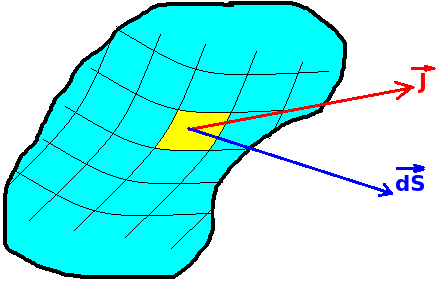
\includegraphics[width=6cm] {obrazek1}
\end{center}
\textit{Rys. 1. Rysunek pomocniczy.}
Spełnione jest:
\begin{equation}
\frac{dQ}{dt}=-\int \vec{dS}\cdot\vec{J}\arg \label{zl}
\end{equation}
gdzie: 
\begin{itemize}
\item $\vec{dS}$ - element powierzchni; $|\vec{dS}|$ - pole powierzchni
\item Q- całkowity ładunek, wyrażający się wzorem:
\begin{equation}Q(t)=\int d^3r \rho\arg \label{Q} \end{equation}
\item $\vec{dS}$  - wektor powierzchni, którego długość jest równa polu powierzchni, 
\item natomiast wyrażenie po prawej stronie to natężenie prądu będące równe strumieniowi przepływającemu przez daną powierzchnię:
\begin{equation}
I(t)=\int \vec{dS}\cdot\vec{J}\arg 
\end{equation}
\end{itemize}
uw. Minus w równaniu (\ref{zl}) oznacza, że ładunek może tylko wypływać spod powierzchni.\\
uw2. Wyrażenie pod całką to strumień prądu płynący przez rozważany obszar.

Wstawmy równanie (\ref{Q}) do równania (\ref{zl}):
\begin{equation}
\partial_t \int_{\partial\Omega} d^3r\rho\arg= -\int_{\partial\Omega}\vec{dS}\cdot\vec{J}\arg 
\stackrel{\text{tw.Gaussa}}{=} -\int_\Omega d^3r\nabla\cdot\vec{J}\arg
\end{equation}
\begin{equation}
\int d^3r\{\partial_t \rho\arg+\nabla \cdot\vec{J}\arg\}=0
\end{equation}
Stąd:
\begin{equation}
\partial_t \rho\arg+\nabla \cdot\vec{J}\arg=0 \label{zl2} \end{equation}
Wzór (\ref{zl2}) to prawo zachowania ładunku - ładunek nie może zniknąć, może tylko przepłynąć przez powierzchnię.

\subsubsection{Wyprowadzenie praw zachowania ładunku z praw Maxwella}
Zadziałajmy obustronnie $\partial_t$ na 1. równanie Maxwella (\ref{r1}) oraz $\nabla\cdot$ na 2. równanie Maxwella (\ref{r2}):
\begin{equation}
(1)~~\Rightarrow ~~\partial_t \nabla\cdot \vec{D}\arg=\delta_t \rho(\r,t) ~~\Rightarrow~~ \nabla\cdot[\partial_t\vec{D}\arg=\partial_t\rho\arg \end{equation}
 \begin{equation}
 (2)~~\Rightarrow~~ \underbrace{\nabla\cdot[\nabla\times\vec{H}\arg]}_{=0 \text{ (bo jest to div z rot)}}-\nabla\cdot\partial_t\vec{D}\arg=\nabla\cdot\vec{J}\arg
\end{equation}
Łącząc oba te równania dostajemy:
\begin{equation}
-\partial_t\rho\arg=\nabla\cdot\vec{J}\arg \label{zz}
\end{equation}
Równanie (\ref{zz}) to zasada zachowania ładunku.

\subsubsection{Równania materiałowe} 
Z jednej strony równania Maxwella są niezmiennicze względem zmiany ośrodka, z drugiej strony ich rozwiązania- pola $\E,\B$- są różne w różnych ośrodkach. Dlatego potrzebujemy dodatkowych równań, które będą określać ośrodek- dlatego postulujemy równania materiałowe:
\begin{equation} {D}_i\arg=\sum_{j/1}^3\int d^3r'\int_{-\infty}^t dt' \epsilon_{ij}\argg E_j \label{rm1}\end{equation}
\begin{equation} H_i \arg =\sum_{j/1}^3\int d^3r'\int_{-\infty}^t dt' \mu^{-1}_{ij}\argg B_j \label{rm2}\end{equation}
\begin{equation} J_i \arg =\sum_{j/1}^3\int d^3r'\int_{-\infty}^t dt' \sigma_{ij}\argg E_j \label{rm3}  \text{ - mikroskopowe prawo Ohma}\end{equation}
\begin{verse}\textbf{wn.1.} Mamy zatem zestaw równań: Równania Maxwella+równania materiałowe \end{verse}
\begin{verse}\textbf{wn.2.} W równaniach materiałowych jądrem całkowym są:\\
(\ref{rm1}): ~ $\epsilon_{ij}\argg$ - to element tensora przenikalności elektrycznej ośrodka\\
(\ref{rm2}):  ~$\mu^{-1}_{ij}\argg$ - to element tensora odwrotności przenikalności magnetycznej\\
(\ref{rm3}):  ~$\sigma_{ij}\argg$  - to element tensora przewodnictwa elektrycznego. \end{verse}
\begin{verse} \textbf{uw.1.} Równania materiałowe mają swoje uzasadnienie w termodynamice stanów nierównowagowych, natomiast do elektrodynamiki zostały dodane \textsl{ad hoc}.
uw.2. \end{verse}
\begin{verse} \textbf{uw.2.} Ostatnie (\ref{rm3}) równanie to mikroskopowe (lokalne) prawo Ohma, które można również zapisać w popularniejszej wersji:
\begin{equation} \vec{J} \arg =\sigma\arg E\arg \end{equation} \end{verse}

\subsubsection{Równania Maxwella a prąd stały}
\begin{verse} \textbf{Zał.} Załóżmy, że \textbf{prąd jest stały}, tzn. płynie w sposób ciągły i nie gromadzi się (jest stały w czasie). \end{verse}

Wówczas:\begin{itemize}
\item Równanie Maxwella (\ref{r2}) $\Rightarrow$ powstaje stałe pole $\vec{H}$
\item Równanie Maxwella (\ref{r3}) $\Rightarrow ~~ \nabla\times\vec{E}(\r)+\underbrace{\partial_t\vec{B}(\r)}_{=0}=0$ \\
Stąd:
\begin{equation} \nabla\times\vec{E}(\r)=0 \end{equation}
Ponieważ wiemy, że dywergencja z rotacji daje 0, to $\vec{E}$ musi dać się przedstawić jako:
\begin{equation} \vec{E}=-\nabla V(\r) \label{Epot}\end{equation}
gdzie $V(\r)$ to potencjał.
\begin{verse} \textbf{wn.} Jeśli prąd jest stały, to pole elektryczne ma potencjał. \end{verse} 
\item Prawo zachowania ładunku (\ref{zl2}) $\Rightarrow ~~ \underbrace{\partial_t\rho\arg}_{=0}+\nabla\cdot\vec{J}\arg=0 $
\begin{equation} \nabla\cdot\vec{J}({\r})=0 \end{equation}
\item Mikroskopowe prawo Ohma $\Rightarrow ~~ \nabla[\sigma(\r)\vec{E}(\r)]=0$ \\
Łącząc to równanie z równaniem (\ref{Epot}), dostajemy: \\ 
\begin{equation} -\nabla \cdot[\sigma(\r) \nabla V(\r)] =0  \nonumber \end{equation}
\begin{equation} \nabla \cdot[\sigma(\r) \nabla V(\r)] =0 \label{doLaplace} \end{equation}
\item Załóżmy teraz, że przewodnictwo jest wszędzie takie samo: $\sigma(\r)=const=\sigma $.\\
Wówczas z równania (\\ref{doLaplace}) wynika:
\begin{equation} \sigma \nabla ^2 V(\r) =0 \end{equation}
O ile $\sigma \neq 0 $ (czyli nie jest to izolator):
\begin{equation} \nabla^2 V(\r)=0\end{equation}
Jest to równania Laplace'a.
\begin{verse} \textbf{wn.} Jeśli prąd jest stały, to potencjał układu spełnia równanie Laplace'a. \end{verse}
\begin{verse} \textbf{uw.} Bez założenia o prądzie stałym dostalibyśmy równanie Poissona \end{verse}
\end{itemize}
\subsubsection{Dygresja - potencjał a energia potencjalna}
Energia potencjalna wyraża się wzorem:
\begin{equation} U(\r) \equiv \int d^3r'\rho(\r')V(\r) \end{equation}
Łącząc powyższe równanie z definicją gęstości ładunkowej:
\begin{equation} U(\r) = \int d^3r'q\delta(\r-\r')V(\r)\end{equation}
Stąd:
\begin{equation} U(\r) = qV(\r) \label{Pot}\end{equation}
Równanie (\ref{Pot}) to związek pomiędzy energią potencjalną a potencjałem.

\section{Zlinearyzowane relacje konstytutywne ośrodków materialnych}
\subsection{Ogólna postać równań materiałowych}
Można zauważyć, że wszystkie równania materiałowe (\ref{rm1}),(\ref{rm2}),(\ref{rm3}) mają postać:
\begin{equation} \vec{Y}(\r,t)=\int d^3r \int_{-\infty}^t dt' \hat{\chi}(\r,\r',t,t') \vec{X}(\r',t') \end{equation}
lub równoważnie:
\begin{equation} {Y}_i(\r,t)=\sum_{j/1}^3 \int d^3r \int_{-\infty}^t dt' {\chi}_{ij}(\r,\r',t,t') X_j(\r',t') \end{equation}
gdzie:\\
\begin{itemize} \item $\vec{Y}$ - wektor reprezentujący pole wtórne
\item $\vec{X}$ - wektor reprezentujący pole pierwotne
\item $\hat{\chi} $ - to tzw. uogólniona podatność (inaczej: funkcja odpowiedzi układu). Jest to tensorowe jądro całkowe, służące do przekształcenia pola pierwotnego we wtórne - zatem wnosi ona informację o ośrodku.
\end{itemize}
\begin{verse}\textbf{uw.}
Dlaczego całka po czasie biegnie do $t$ a nie do $\infty$? \\
Ponieważ wówczas $\chi$ zbiera informacje do chwili obecnej. Gdyby całka była do $\infty$, to złamalibyśmy \textbf{zasadę przyczynowości} (wyraża ona, że skutek obserwowany w chwili obecnej zależy tylko do przyczyn z przeszłości). \\
Można zatem postawić:
\begin{equation}\chi_{ij}(\r,\r',t,t')=0 \text{ ~~~~dla~ } t'>t\end{equation}
\end{verse}

\subsection{Równania materiałowe a teoria liniowej odpowiedzi}
\textbf{Fakty:}
\begin{enumerate}
\item Pola wtórne są liniowymi funkcjonałami pól pierwotnych:
\begin{equation} \vec{Y}[\alpha_1\vec{X}_1 + \alpha_2\vec{X}_2]=\alpha_1 \vec{Y}[\vec{X}_1] + \alpha_2 \vec{Y}[\vec{X}_2] \end{equation}
\textbf{uw.} Jeśli uciąglimy tę sumę, dostaniemy całkę.
\item Równania materiałowe pozostają słuszne, jeśli pola pierwotne można traktować jako słabe zaburzenia. Wówczas można rozwinąć w szereg McLaurina:
\begin{equation}\vec{Y}[\vec{X}]=\vec{Y}[\vec{0}]+ \frac{\delta\vec{Y}}{\delta\vec{X}}|_{\vec{0}}\vec{X} + \frac{1}{2}\frac{\delta^2 \vec{Y}}{\delta\vec{X}^2}|_{\vec{0}}\vec{X}^2 + ...\end{equation}
gdzie: $\vec{Y}[\vec{0}]=0$ (bo nie może istnieć pole wtórne bez pierwotnego), zatem:
\begin{equation}[\vec{X}]=\vec{Y}[\vec{0}]+ \frac{\delta\vec{Y}}{\delta\vec{X}}|_{\vec{0}}\vec{X} + \mathcal{O}(\vec{X}^2)\end{equation}
\end{enumerate}
\textbf{Założenie:}\begin{verse} 
Załóżmy, że pola wtórne są proporcjonalne do pól pierwotnych (tzw. linearyzacja równania). Wówczas:
\begin{equation}\vec{Y}[{\vec{X}}] \simeq \frac{\delta\vec{Y}}{\delta\vec{X}}|_{\vec{0}} \vec{X} = \hat{\mathcal{L}}\vec{X}\end{equation} \end{verse}
Ostatecznie więc:
\begin{equation}\vec{Y}[{\vec{X}}] = \hat{\mathcal{L}}\vec{X} \label{RFen} \end{equation}
To przybliżenie nazywamy \textbf{teorią liniowej odpowiedzi}, zaś samo równanie (\ref{RFen}) - równaniem fenomenologicznym, a współczynniki $\hat{\mathcal{L}}$ - współczynnikami fenomenologicznymi. Współczynniki te dostajemy z doświadczeń i następnie staramy się je wyjaśnić za pomocą teorii.

\subsection{Uogólnienie na wiele pól zaburzających - zjawiska krzyżowe}
Z racji liniowości wektora $\vec{Y}$, równanie (\ref{RFen}) można uogólnić na wiele pól zaburzających (np. możemy jednocześnie rozważać pola $\B$ i $\E$) :
\begin{equation} \vec{Y}=\hat{\mathcal{L}}\vec{X} \arg 
\stackrel{\text{uogólnienie}}{\longrightarrow}  {Y}_i=\sum_{j/1}^n \mathcal{L}_{ij} X_j \end{equation}
\begin{verse} \textbf{Np.} Niech n=2. Wówczas:
\begin{center} 
$\begin{cases} \vec{Y}_1=\mathcal{L}_{11}\vec{X}_1+\mathcal{L}_{12}\vec{X}_2 ~~~~~~~~~~/\mathcal{L}_{12}^{-1}\\ \vec{Y}_2=\mathcal{L}_{21}\vec{X}_1+\mathcal{L}_{22}\vec{X}_2 ~~~~~~~~~~/\mathcal{L}_{22}^{-1}
\end{cases}$
\end{center}

\textbf{wn.} Pole wtórne wynika z obu pól pierwotnych.\\
Wyznaczamy $\vec{X}_1$:
\begin{center}
$\begin{cases} \mathcal{L}_{12}^{-1}\vec{Y}_1=\mathcal{L}_{12}^{-1}\mathcal{L}_{11}\vec{X}_1+\vec{X}_2 \\ \mathcal{L}_{22}^{-1}\vec{Y}_2=\mathcal{L}_{22}^{-1}\mathcal{L}_{21}\vec{X}_1+\vec{X}_2 
\end{cases}$
\end{center}
Odejmując stronami, dostajemy:
\begin{equation} \mathcal{L}_{12}^{-1}\vec{Y}_1 - {L}_{22}^{-1}\vec{Y}_2 = [\mathcal{L}_{12}^{-1}\mathcal{L}_{11} - \mathcal{L}_{22}^{-1}\mathcal{L}_{21}]\vec{X}_1 \nonumber \end{equation}
\begin{equation} 
 [\mathcal{L}_{12}^{-1}\mathcal{L}_{11}-\mathcal{L}_{22}^{-1}\mathcal{L}_{21}]^{-1} \mathcal{L}_{12}^{-1}\vec{Y}_1 -   
 [\mathcal{L}_{12}^{-1}\mathcal{L}_{11} - \mathcal{L}_{22}^{-1}\mathcal{L}_{21}]^{-1} \mathcal{L}_{22}^{-1}\vec{Y}_2 =\vec{X}_1  \nonumber \end{equation}
 
\textbf{wn.} Pole pierwotne $\vec{X}_1$ można przedstawić w postaci kombinacji liniowej pól wtórnych, przy czym $\vec{X}_1$ produkuje $\vec{Y}_1$ oraz $-\vec{Y}_2$. Zauważmy, że $\vec{Y}_2$ jest z minusem, bo przeciwdziała ono polu $\vec{Y}_1$.\\ ~~~~Takie procesy z polami $\vec{Y}_1$ i $\vec{Y}_2$ naz. zjawiskami krzyżowymi.\\
\textbf{np.} W zjawiskach termoelektrycznych polami tymi są $\vec{E}$ i gradient temperatury $\nabla T$: Pole elektryczne przemieszcza elektrony, ale przez opór materiał się grzeje, więc powstaje gradient temperatury.
\end{verse}
\subsection{Klasyfikacja materiałów ze względu na jądro całkowe równania materiałowego}
\begin{enumerate}
\item Ośrodek materialny jest \textbf{lokalnie liniowy} wtedy i tylko wtedy, gdy $\hat{\chi}$ ma postać:
\begin{equation}\hat{\chi}(\r,\r',t,t')=\hat{\chi}(\r',t,t')\delta(\r-\r')\end{equation}
\item Ośrodek materialny jest \textbf{przestrzennie jednorodny} wtedy i tylko wtedy, gdy $\hat{\chi}$ ma postać:
\begin{equation}\hat{X}(\r,\r',t,t')=\hat{\chi}(\r-\r',t,t')\end{equation}
Jeśli równość ta nie zachodzi, to ośrodek jest \textbf{niejednorodny przestrzennie}.
\item Ośrodek materialny jest \textbf{czasowo jednorodny} wtedy i tylko wtedy, gdy $\hat{\chi}$ ma postać:
\begin{equation}\hat{\chi}(\r,\r',t,t')=\hat{\chi}(\r,\r',t-t')\end{equation}
 Np. gdy materiał się grzeje, to w różnych chwilach różne jest pole $\nabla T$
 Jeśli równość ta nie zachodzi, to ośrodek jest \textbf{niejednorodny czasowo}.
 \item Ośrodek materialny jest \textbf{czasowo i przestrzennie jednorodny} wtedy i tylko wtedy, gdy $\hat{\chi}$ ma postać:
\begin{equation}\hat{\chi}(\r,\r',t,t')=\hat{\chi}(\r-\r',t-t')\end{equation}
 Tę własność spełnia gaz elektronowy oraz nukleony w jądrze.
  \item Ośrodek materialny jest \textbf{izotropowy} wtedy i tylko wtedy, gdy elementy macierzowe $\hat{\chi}$ mają postać:
\begin{equation}{\chi}_{ij}(\r,\r',t,t')=\hat{\chi}(\r-\r',t-t')\delta_{ij}\end{equation}
 Jeśli równość ta nie zachodzi, to ośrodek jest \textbf{anizotropowy}.
 \item Ośrodek materialny jest \textbf{homogeniczny} wtedy i tylko wtedy, gdy elementy macierzowe $\hat{\chi}$ mają postać:
\begin{equation}{\chi}_{ij}(\r,\r',t,t')={\chi}\delta(\r-\r')\delta(t-t')\delta_{ij}\end{equation}
\end{enumerate}
\subsection{Równanie materiałowe dla ośrodka homogenicznego- konsekwencje}
Wróćmy do równania materiałowego:
\begin{equation} {Y}_i(\r,t)=\sum_{j/1}^3 \int d^3r \int_{-\infty}^t dt' {\chi}_{ij}(\r,\r',t,t') X_j(\r',t') \end{equation}
W ośrodku homogenicznym:
\begin{equation} {Y}_i(\r,t)=\sum_{j/1}^3 \int d^3r \int_{-\infty}^0 dt' {\chi}\delta(\r-\r')\delta(t-t')\delta_{ij} X_j(\r',t')\arg 
\stackrel{\text{tw.filtracyjne}}{=}\chi X_i(\r,t) \end{equation}
Zatem:\\
\begin{center}
%\caption{fsdF}
\begin{tabular}{|c||c|c|}
  \hline
 ${_Y^~~X}$ & $\vec{E}$ & $\vec{B}$\\
  \hline\hline
  $\vec{D}$ &  $\hat{\epsilon}$ & brak \\
\hline
  $\vec{H}$ &  brak & $\hat{\mu}^{-1}$ \\
  \hline
  $\vec{J}$ &  $\hat{\sigma}$ &  brak\\
    \hline
\end{tabular} 
\end{center}
\textbf{wn. 1.} Z powyższego wynika mikroskopowe prawo Ohma dla ośrodków homogenicznych: \begin{equation} \vec{J}(\r,t)=\sigma\E \end{equation}
Zatem Ohm miał szczęście, że przykładał małe pola (bo w powyższych rachunkach zastosowaliśmy rachunek zaburzeń prawdziwy dla małych pól).\\
\textbf{wn. 2.} Dla układów homogenicznych skalarna stała $\chi$ reprezentuje stałą materiałową, która opisuje w sposób ilościowy rozpatrywaną własność ośrodka.
\subsection{Punkt widzenia}
Ustalmy jeden z dwóch możliwych punktów widzenia:
prąd elektryczny jest konsekwencją przyłożonego pola elektrycznego $\E$. Pole elektryczne to przyczyna, a prąd to skutek.

\section{Metody opisu klasycznej dynamiki cząstek}
W rozważaniach opuszczamy mechanikę Lagrangowską. 
\subsection{Mechanika newtonowska}
\textbf{Siła Lorenza}
\begin{equation}\label{sila_lorenza}
	\vec{F}_l \arg = q [ \vec{E} \arg+\vec{v}(t)\times\vec{B}\arg].
\end{equation}
Jeżeli postać siły jest określona, to równanie ruchu możemy 
zapisać w postaci
\begin{equation}
	m\frac{d^2\vec{r}(t)}{dt^2}=\vec{F}_L \arg  .
\end{equation}
Zauważmy, że w mechanice Newtonowskiej nie ma ograniczenia na 
postać siły $\vec{F}_L$.
\textbf{Przykład - równanie Langevine'a}
$$ m\frac{d^2}{dt^2} \vec{r}(t) = \vec{F}_R - \gamma\vec{v}(t) +
\vec{\Gamma}(t),$$
gdzie $\vec{F}_R$ to siła regularna (np. od zewnętrznego pola 
elektrycznego, $\gamma$ to współczynnik tarcia, a $\vec{\Gamma(t)}$ 
to siła stochastyczna.
Rozwiązując równania Newtona otrzymujemy różne $\vec{r}(t)$. 
Oznaczmy przez $\{ \vec{r}(t) \}$ - zbiór rozwiązań równania Newtona
$\equiv$ PRZESTRZEŃ KONFIGURACYJNA.

RYSUNEK


$\left|\vec{r}(t)\right> $ - klasyczny stan cząstki w mechanice Newtona 
niewystarczający ze względu na brak determinizmu.

Stan cząstki opisany w spsób (trik dodający determinizm) $$\left| \vec{r}(t)
,\vec{v}(t) \right> \mbox{ - klasyczny stan cząstki}$$
$$
\begin{cases} 
	\dt \vec{r}(t)=\vec{v}(t) &\\
	m\dt \vec{v}(t)=\vec{F}(\vec{r},t)
\end{cases} + \mbox{war. początkowe (jednopunktowe)} 
\begin{cases}
	\vec{r}(t_0)=\vec{r}_0
	\vec{v}(t_0)=\vec{v}_0
\end{cases}
$$
\textbf{Uwaga}\\
Możemy określić $\vec{r}$ w chwili $t$, ale $\vec{v}$ okreśamy w otoczeniu $t$,
bo
$$\vec{v}_0 = \vec{v}(t_0) = \dt \vec{r}_{\Big|_{t=t_0}} = \lim_{\Delta t \to 0}
\frac{\vec{r}(t_0+\Delta t)-\vec{r}(t_0)}{\Delta t},$$
ewentualnie
$$\vec{v}_0 = \vec{v}(t_0) = \dt \vec{r}_{\Big|_{t=t_0}} = \lim_{\Delta t \to 0}
\frac{\vec{r}(t_0)-\vec{r}(t_0-\Delta t)}{\Delta t}.$$
\textbf{Wniosek}\\
Trikiem Tym uzyskujemy determinizm, z wyjątkiem infinitezymalnych zmian.

\subsection{Mechanika hamiltonowska}
W mechanice hamiltonowskiej nie używamy pojęcia siły, ale pojęcia potencjału,
co oznacza, że jest ona mniej ogólna.\\

\textbf{formalizm kanoniczny}\\
Funkcja Hamiltona: $ H\qpt$. Kosztem straty na ogólności, zyskujemy 
niezależność zmiennych uogólnionych $\vec{q}$ i $\vec{p}$.\\
$$ \left| \vec{q}(t), \vec{p}(t) \right> \mbox{ - klasyczny stan układu.} $$
Funkcja Hamiltona przybiera wartość całkowitej energii mechanicznej układu, jeżeli
siły sziałające na układ są potencjalne, a potencjał nie zależy od czasu.
$$ H\qp = \underbrace{J(\vec{q},\dot{\vec{q}}(\vec{q},\vec{p}))}_{\mbox{
część kinetyczna}} + \underbrace{U(\vec{q})}_{\mbox{część potencjalna}}.$$

\section{Metody Statystyczne w układach wielocząstkowych}
\subsection{Model klasycznego gazu doskonałego}
\subsubsection{Wstęp}
Pamiętamy, że dynamiczę cząstek naładowanych w polu EM można obliczyć poprzez:
\begin{itemize}
\item rozwiązanie równania Newtona
\item hamiltonowską metodę, gdzie zaletą jest fakt, że położenie i pęd są niezależnymi zmiennymi
\end{itemize}
Dla N cząstek powinniśmy rozwiązać N równań ruchu. Gdy $N\rightarrow\infty$, to problem staje się nieobliczeniowy (nie da się go obliczyć w skończonym czasie).\\
Rozwiązanie tego problemu: użycie statystyki do obliczeń (fizyka statystyczna). Okazało się, że metody statystyczne poprawnie działają dla dużych układów. Cena za to: utrata jednoznaczności niektórych pojęć. Zysk: problem staje się obliczeniowy; przy okazji ujawniły się niektóre zależności statystyczne. 
\subsubsection{Definicja}
\begin{verse}\textbf{Df.} Klasycznym gazem doskonałym naz. układ cząstek punktowch, między którymi nie ma żadnego oddziaływania \end{verse}
\begin{verse}\textbf{uw.} W df. na Wikipedii mamy jeszcze zawarte, że układ ten osiąga równowagę termodynamiczną natychmiast w wyniku zderzeń- to nie jest prawda. W defininicji klasycznego gazu doskonałego zakładamy brak zderzeń, czyli układ jest niestabilny termodynamicznie \end{verse}
\subsubsection{Stała Schmidta}
Stała Schmidta odpowiada na pytanie ile jest cząstek w $1 cm^3$ gazu w warunkach normalnych:
\begin{equation}\text{STAŁA SCHMIDTA}=\frac{\text{L. AVOGADRO}}{\text{OBJĘTOŚĆ 1 MOLA GAZU}}\end{equation}
czyli:
\begin{equation}n_0=\frac{N_A}{V}=\frac{6.02214\cdot 10^{23} ~{1/mol}}{22413.19 ~cm^3/mol}=2.68678\cdot 10^{19} cm^{-3} \simeq 3\cdot 10^{19} \frac{\text{cząstek}}{cm^3}\end{equation}
\subsubsection{Rozwiązanie równań ruchu metodą Hamiltona}
\begin{itemize}
\item Funkcja Hamiltona:
\begin{equation}H(\{\r_i\},\{\p_i\})=\sum_{i/1}^{N}\frac{p_i^2}{2m}\end{equation}
\item Równania ruchu dla tej funkcji:
\begin{equation}\begin{cases} \dt \r_j(t)=\nabla_{\p_j} H(\{\r_i\},\{\p_i\})=\sum_{i/1}^{N}\frac{\p_j(t)}{m}\delta_{ij}=\frac{1}{m}\p_j(t)\\ \dt\p_j(t)=-\nabla_{\r_j} H(\{\r_i\},\{\p_i\})=0\end{cases}\end{equation} 
\item Warunki brzegowe:
\begin{equation}\begin{cases} \r_j(t=0)=\r_{j0} \\ \p_j(t=0)=\p_{j0}\end{cases}\end{equation}
\item Po scałkowaniu równań ruchu dostajemy:
\begin{equation}\begin{cases} \r_j(t)=\r_{j0}+\frac{1}{m}p_{j0}t\\ \p_j(t)=p_{j0}\end{cases} \label{RRuchu}\end{equation}
\begin{verse}\textbf{Wn.} Każda z N cząstek gazu doskonałego ewoluuje niezależnie od pozostałych\end{verse}
\begin{verse}\textbf{Wn.} Pęd cząstki w tym gazie jest stały \end{verse}
\end{itemize}
\subsubsection{Cząsteczkowa przestrzeń fazowa $\mu$}
\begin{verse}\textbf{Df.} Cząsteczkowa przestrzeń fazowa $\mu$ to przestrzeń 6-wymiarowa:\\
\begin{center}dim[$\mu$]=6 \end{center}
w której ruch wyznaczają 2 niezależne zmienne:\\
\begin{center}$|\r_j(t),\p_j(t)>$\end{center}\end{verse}
Zatem dowolny punkt należący do tej przestrzeni to:
\begin{equation}\vec{a}\epsilon\mu~:~\vec{a}=(x,y,z,p_x,p_y,p_z)\end{equation}
Czyli 1 punkt to jedna cząsteczka.
\begin{verse}\textbf{Np.} Aby to narysować, upraszczamy problem do układu 1D+1D:\\
\begin{center}$dim[\mu]=2$\\
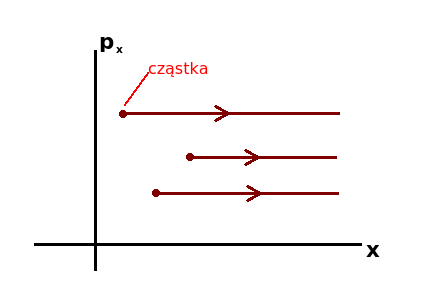
\includegraphics[scale=0.75] {obrazki/przestrzen_fazowa1.png}
\end{center}
\textbf{Uw.} Cząstki nie mogą być ułożone na 1 linii równoległej do osi pędowej, bo wtedy byłyby w 1 punkcie przestrzennym.
\end{verse}
\subsubsection{Opis gruboziarnisty}
Problem: potrzeba 2N warunków brzegowych.
Rozwiązanie: opis grupoziarnisty:\\
Wybierzmy element objętości przestrzeni $\mu$ wokół punktu L o objętości $[|\Delta \r_l|]^3$:
\begin{center}$dim[\mu]=2$\\
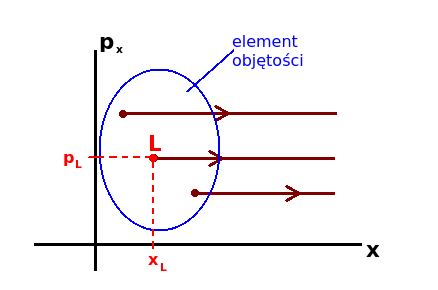
\includegraphics[scale=0.75] {obrazki/przestrzen_fazowa2.png}
\end{center}
Jeśli punkt:
\begin{equation} (\r_L,\p_L)\epsilon\mu~ \nonumber \end{equation}
wtedy element objętości:
\begin{equation}\Delta\omega_L=\Delta\r_L\Delta\p_L\end{equation}
przy czym wymiar elementu objętości jest rzędu długości, po której średniowaliśmy na poprzednich wykładach:
\begin{equation}|\Delta\r_L\sim L\sim 100nm\end{equation}
W kostce o takich rozmiarach liczba cząstek wynosi:
\begin{equation}[|\Delta\r_L|]^3[n_0 cm^{-3}]=[10^{-5}cm]^3[3\cdot10^{19}cm^{-3}]=3\cdot 10^4 \text{cząstek}\nonumber\end{equation}
Opis ten nazywamy opisem gruboziarnistym, ponieważ każdy element objętości dobieramy sobie dowolnie.

\subsection{Funkcja rozkładu gęstości prawdopodobieństwa}
\subsubsection{Definicja}
Wprowadźmy funkcję pomocniczą:
\begin{center}$\f$\end{center}
Żądamy, by była ona klasy $C^0[\mu]$, czyli by była ciągła w przestrzeni $\mu$.
Wyrażenie:
\begin{equation}\f\Delta\omega_L\end{equation}
opisuje liczbę cząstek w objętości $\Delta\omega_L$, w której położenia i prędkości zmieniają się zgodnie z rozkładem f.\\
Umówmy się, że:
\begin{equation}
\begin{cases} \sum_L f(\r_L,\p_L,t)\Delta\omega_L=\int d^3 r d^3 p\f \\ \int d^3r d^3p\f=N~\Rightarrow\text{f jest unormowana do liczby cząstek}\end{cases}
\end{equation}
Wówczas $\f$ jest \textbf{funkcją rozkładu gęstości prawdopodobieństwa}.
\subsubsection{Równanie kinetyczne dla tej funkcji}
\begin{itemize}
\item{Wyprowadzenie równania kinetycznego}\\
Zauważmy, że:
\begin{equation}f(\r,\p,t+dt)-\f \stackrel{\text{ciągłość f}, dt\rightarrow 0}{\simeq}\partial_t\f dt\end{equation}
gdzie
\begin{equation}\partial_t\equiv \frac{\partial}{\partial t}\end{equation}
W czasie dt położenie i pęd zmieniają się jak:
\begin{equation}d\r(t)=\dot{\r}(t)dt \end{equation}
\begin{equation} d\p(t)=\dot{\p}(t)dt \stackrel{\text{r.(\ref{RRuchu})}}{=}0\end{equation}
Wtedy:
\begin{equation}\f-f(\r+d\r,\p,t)\simeq -\dot{\r}(t)\nab{r}\f dt=-\frac{1}{m}\p(t)\nab{r}\f dt\end{equation}
i oczywiście:
\begin{equation}\f-f(\r,\p+d\p,t)\simeq -\dot{\p}(t)\nab{p}\f=0 \end{equation}
Zatem:
\begin{equation}\frac{d\f}{dt}=\partial_t\f+\frac{1}{m}\p(t)\cdot\nab{r}\f=0 \label{Rkinet}\end{equation} 
\textbf{Moja uwaga}: To zwykła "reguła łańcuchowa":
\begin{equation} \frac{d\f}{dt}=\frac{\partial\f}{\partial\r}\frac{\partial\r}{\partial t}+\frac{\partial\f}{\partial\p}\frac{\partial\p}{\partial t}+\frac{\partial\f}{\partial t}=\dot{r}(t)\nab{r}\f+0+\partial_t\f\end{equation}
Wiemy, że:
\begin{equation}mv(\p(t))=\p(t)~~ \Rightarrow ~~\vec{v}(\p(t))\equiv\v(\p)=\frac{1}{m}\p(t)\end{equation}
Wówczas równanie (\ref{Rkinet}) ma postać:
\begin{equation}\partial_t\f+\v(\p)\cdot\nab{r}\f=0\label{Rkinet2}\end{equation}
Powyższe równanie to \textbf{równanie kinetyczne}.
\item{Rozwiązanie równania kinetycznego}\\
Postulujemy rozwiązanie tego równania:
\begin{equation}\f=\Phi(\r-\v t,\p)\end{equation}
gdzie $\Phi$ to dowolna funkcja klasy $C^0[\mu]$.\\
Dowód, że jest to rozwiązanie:
\begin{verse}\textbf{ Ozn. }
\begin{equation} \vec{s}(t)=\r(t)-\v(t)\end{equation} \end{verse}
Wówczas kolejne części równania kinetycznego zyskują postać:
\begin{equation}\begin{cases} \Phi(\r-\v t,\p)~~\rightarrow ~~ \tilde{\Phi}(\vec{s}(t),\p) \\ 
\partial_t\Phi(\r(t)-\v t,\p)=\frac{\partial\vec{s}(t)}{\partial t}\nab{s}\tilde{\Phi}(\vec{s}(t),\p) \\ 
\nab{r}\Phi(\r(t)-\v t,\p)=\nab{r}\vec{s}t)\cdot\nab{s}\tilde{\Phi}(\vec{s}(t),\p)=\nab{s}\tilde{\Phi}(\vec{s}(t),\p) \end{cases}\end{equation}
Zatem równanie kinetyczne przyjmuje postać:
\begin{equation}\{-\v\cdot\nab{s}+\v\cdot\nab{s}\}\tilde{\Phi}(\vec{s}(t),\p)=0\end{equation}
Obie strony są równe, więc zaproponowana postać rozwiązania jest słuszna.
\end{itemize}
\subsubsection{Momenty funkcji rozkładu gęstości prawdopodobieństwa}
\begin{itemize}
\item {Zerowy moment}\\
\begin{equation}\int d^3p\f=n\arg\end{equation}
to zerowy moment funkcji rozkładu gęstości prawdpodobieństwa. Jest to jednocześnie rozkład brzegowy w przestrzeni położeniowej.
\item {Pierwszy moment}\\
Scałkujmy równanie kinetyczne (\ref{Rkinet2}) po pędzie:
\begin{equation}\partial_t\f+\v(\p)\cdot\nab{r}\f=0~~~~~~/\int d^3 \p\nonumber \end {equation}
\begin{equation}\partial_t n\arg+\int d^3\p ~\v(\p)\cdot\nab{r}\f=0 \nonumber\end{equation}
Pamiętamy, że wyszliśmy z hamiltonianu, w którym zmienne $\r,\p$ są niezależne (jesteśmy w przestrzeni $\mu$, zatem:
\begin{equation}\partial_t n\arg+\nab{r}\int d^3\p~\v(\p)\f=0 \nonumber\end{equation}
gdzie:
\begin{equation}\vec{j}\arg=\int d^3\p~\v(\p)\f\end{equation}
to pierwszy moemnt funkcji rozkładu gęstości prawdopodobieństwa. Jest on interpretowany jako prąd.
\end{itemize}
\subsubsection{Interpretacja}
\begin{itemize}
\item{Równanie kinetyczne jako równanie ciągłości}\\
Równanie kinetyczne wyrażone przez momenty ma postać:
\begin{equation}\partial_t n\arg+\nab{r}\j\arg=0\end{equation}
W ten sposób nadaliśmy równaniu kinetycznemu strukturę \textbf{równania ciągłości} ("nic nie może zginąć").
\item{Funkcja rozkładu gęstości prawdopodobieństwa wyrażona przez deltę Diraca}\\
Z definicji:
\begin{equation}\j\arg=\int d^3 p~\v(\p)\f\end{equation}
Z drugiej strony, w teorii Lorentza założyliśmy, że prąd cząsteczkowy ma postać:
\begin{equation}\j\arg=\sum_{i/1}^N\v_i(t)\delta(\r-\r_i(t))\end{equation}
Łącząc oba fakty, dostajemy:
\begin{equation}\f=const\cdot\sum_{i/1}^N\delta(\r-\r_i(t))\delta(\p)
\end{equation}
\textcolor{red}{!! Ale wtedy:
\begin{equation}\j\arg=const \int d^3p~\v(\p)\sum_{i/1}^N\delta(\r-\r_i(t))\delta(\p)\end{equation}
\begin{equation}\j\arg= const \int d^3p~\v(\p) \delta(\p) \sum_{i/1}^N\delta(\r-\r_i(t))
\end{equation}
\begin{equation}\j\arg=const~\v(\p=\vec{0}) \sum_{i/1}^N\delta(\r-\r_i(t))
\end{equation}}
Ile wynosi const.?
\begin{equation}\f=const\cdot\sum_{i/1}^N\delta(\r-\r_i(t))\delta(\p)~~~/\int d^3rd^3p \nonumber \end{equation}
\begin{equation}N=const\cdot N \nonumber \end{equation}
\begin{equation}const=1 \nonumber \end{equation}
Zatem:
\begin{equation}\f=\sum_{i/1}^N\delta(\r-\r_i(t))\delta(\p) \end{equation}
Ale:
\begin{equation}\r_i(t)=\r_{i0}+\frac{1}{m}\p_{i0}t=\r_{i0}+\v_{i0}t\end{equation}
zatem ostatecznie:
\begin{equation}\f=\sum_{i/1}^N\delta(\r-[\r_{i0}+\v{i0}t])\delta(\p) \end{equation}
\item{Interpretacja}\\
\begin{center}
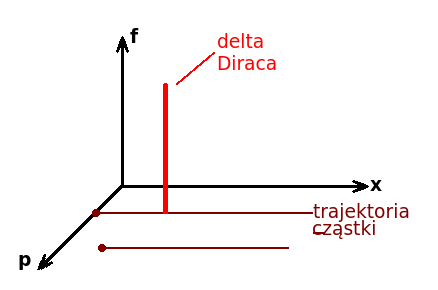
\includegraphics[scale=0.75]{obrazki/przestrzen_fazowa3.png}
\end{center}
Funkcja rozkładu gęstości prawdopodobieństwa przemieszcza się jako delta Diraca wzdłuż trajektorii fazowej w przestrzeni $\mu$ będącej rozwiązaniem kanonicznych równań Hamiltona.\\
\begin{verse}\textbf{Wn. }Założyliśmy brak zderzeń i dostaliśmy to:
\begin{center}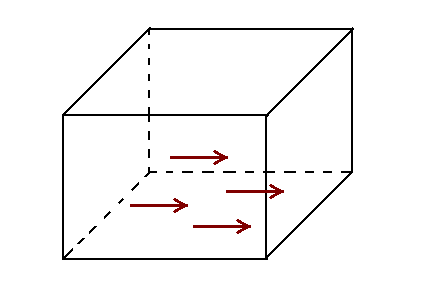
\includegraphics[scale=0.75]{obrazki/przestrzen_fazowa4.png}\end{center}
czyli prąd. \end{verse}
\end{itemize}


\section{Kinetyka fizyczna}
\subsection{Równania transportowe Własowa [Vlasova] i Boltzmana}
Funkcja rozkładu $\f$ na przestrzeni $\mu,\ \dim[\mu]=6.$
\begin{equation} \f d^3rd^3p = \f d^6\omega \implies d^6\omega 
= d^3rd^3p \end{equation}
\begin{equation} \int d^3rd^p\f = N(t) \end{equation}
Dalej dla uproszczenia piszemy samo $N$ pamiętając o zależności czasowej.\\

\textbf{Dla gazu \underline{jednorodnego}:}
$$ \int d^3rd^3p \f = \int d^3rd^3pf(\vec{p},t) = V \int d^3p f(\vec{p},t)=N.$$
\begin{equation}
\int d^3p f(\vec{p},t) = \frac{N}{V} = n \mbox{ - koncentracja cząstek.}
\end{equation}
Oraz
\begin{equation}
N = \frac{\mbox{objętość układu}}{\mbox{objętość na jedną cząstkę}} \equiv 
\frac{V}{v}.
\end{equation}
Dla małego układu 
\begin{equation}
v=\frac{4}{3} \pi r_s^3 ,
\end{equation}
gdzie $r_s$ to promień kulki w jakiej możemy zamknąć jedną cząstkę. Stąd
$$ n = \frac{V}{v} \implies v=\frac{V}{N} = \frac{1}{n}$$
$$ \frac{4}{3} \pi r_s^3 = \frac{1}{n} \implies r_s = \left[ \frac{3}{4\pi n}
\right]^{1/3} \propto n^{-1/3}.$$
\begin{center}
\begin{minipage}{0.3\textwidth}
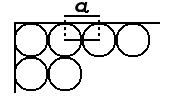
\includegraphics[width=5cm]{kuleczki_z_atomami.png}
\end{minipage}
\begin{minipage}{0.4\textwidth}
średnia odległość $a=2r_s$ \\
między cząsteczkami w gazie \\
o koncentracji $n$ \\
$$a \propto n^{-1/3}$$ \vspace{-5mm}\\
\end{minipage}
\end{center}

\textbf{Dla gazu \underline{niejednorodnego}:}
\begin{equation}
\int d^3rd^3\f = \int d^3r n(\vec{r}) = N \implies n(\vec{r}) 
\mbox{ - gęstość cząstek w } \vec{r}.
\end{equation}

Funkcja rozkładu $f\rpt$. 

Zmiana położenia: efekty dryfowe

Zmiana pędu: efekty polowe

(pomijamy zderzenia)

$$ \Delta t:
\begin{cases} r \to & r+\Delta r \\
				p \to & p+\Delta p\end{cases}$$
$$ f(\vec{r}+\Delta\vec{r},\vec{p}+\Delta\vec{p},t+\Delta t) \simeq 
f\rpt +\nab{r} f\rpt \Delta r + \nab{p} f\rpt + \partial_t f\rpt .
\dfrac{f(\vec{r}+\Delta\vec{r},\vec{p}+\Delta\vec{p},t+\Delta t)-f\rpt}{\Delta t}
\simeq \nab{r} f\rpt \frac{\Delta r}{\Delta }
$$
\subsection{Zespoły statysyczne i przestrzeń fazowa $\Gamma$}


\section{Półklasyczna teoria przewodnictwa elektronowego metali}
\subsection{Zdegenerowany gaz elektronowy}
 \subsubsection{Wstęp}
 W 1926 roku Pauli opublikował zakaz Pauliego, a Fermi i Dirac- statystyki dla elektronów. Statystyki są zupełnie inne od tych, które założył Drude (w statystykach Fermiego-Diraca elektrony mają prędkość zgodnie z rozkładem Maxwella).\\
 W 1927 roku Sommerfeld zmodyfikował teorię Drudego, zakładając w nim statystykę Fermiego- Diraca. Jest to tzw. półklasyczna (a nie kwantowa) teoria, ponieważ Sommerfeld założył kwantową statystykę Fermiego-Diraca, w sposób kwantowy opisał również prawdopodobieństwo przejść, natomiast cały aparat matematyczny pozostał klasyczny.
\subsubsection{Zakaz Pauliego}
\begin{enumerate}
\item \textbf{Tw.} Zakaz Pauliego\\ Prawdopodobieństwo znalezienia w układzie \emph{jednorodnych i nieoddziałujących} fermionów pary cząstek o jednakowych liczbach kwantowych jest równe 0.\\
 \item Komentarz:
\begin{itemize}
\item \emph{nieoddziałujących}- bo jest to gaz elektronowy. Zakładamy, że jest tak rzadki, że nie ma w nim zderzeń elektron-elektron. Są za to zderzenia elektron-jon (jest to zatem gaz Lorentza).
\item\emph{ jednakowych}- nie możemy rozróżnić elektronów- bo zgodnie z mechaniką kwantową nie możemy określić dokładnie ich trajektorii.\\
Przykład: Rozważmy 2 cząstki. O ile w pierwszej chwili możemy określić ich położenie (są to dwa gaussiany; patrz- rysunek poniżej), to w następnych chwilach   ich rozkłady się przekrywają i nie jesteśmy w stanie ustalić położenia danej cząstki - stąd nie możemy określić trajektorii żadnej z tych cząstek.\\
Ewolucję czasową tych 2 cząstek przedstawia poniższy rysunek.
\begin{center}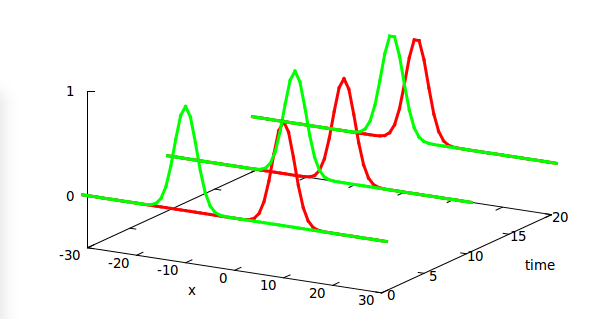
\includegraphics[scale=0.75]{obrazki/wykl_7_obrazek_1.png}\end{center}
To powoduje, że gaz ten nie jest już klasyczny. Jest to tzw. gaz zdegenerowany.
\end{itemize}
\end{enumerate}

\subsubsection{Stan układu- liczby kwantowe}
\begin{itemize}
\item Stan układu
Klasyczny stan układu jest określony przez:
\begin{equation} \left.|\r,\p\right>z\end{equation}
Kwantowy stan układu jest określony przez:
\begin{equation} \left.|\Psi\right>\end{equation}
\item Pęd jako liczba kwantowa
gdzie $\Psi$ to abstrakcyjny wektor stanu.\\
Funkcja falowa przedstawia się wzorem:
\begin{equation}\Psi_{\p}\arg=\frac{1}{V}e^{-\frac{i}{\hbar}(E(\p)t-\p\cdot\r)}\end{equation}
gdzie $\p$ jest liczbą kwantową, bo jednoznacznie określa funkcję falową. Można zatem oznaczać:
\begin{equation} \Psi_{\p}\arg=\left< \r|\Psi_{\p(t)}\right>=\left< \r|\p\right>\end{equation}
gdzie $\left.|\Psi_{\p(t)}\right>$ to wektor stanu zapisany w obrazie Schroedingera.\\
\item Spin jako liczba kwantowa
Kolejną liczbą kwantową jest rzut spinu $\sigma$. Można zatem zapisać:
\begin{equation}\left.|\Psi\right>=\left.|\p,\sigma\right>\end{equation}
\end{itemize}
\subsubsection{Poziomy energetyczne}
Relacja de Broglie'a przedstawia:
\begin{equation}\p=\hbar\ka\end{equation}
gdzie k jest dyskretne:
\begin{itemize}
\item sztywne warunki brzegowe:
\begin{equation} k_i=\frac{n_i\pi}{L_i}~~~~;n_i\epsilon\mathbb{N}\end{equation}
\item periodyczne warunki brzegowe
\begin{equation} k_i=\frac{2n_i\pi}{L_i}~~~~;n_i\epsilon\mathbb{Z}\end{equation}
\end{itemize}
Warunki te przedstawia schematycznie poniższy rysunek:
\begin{center}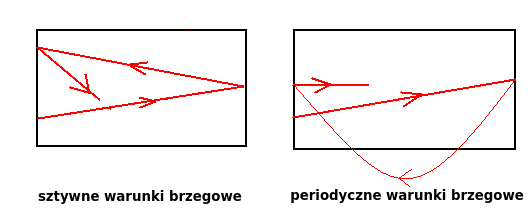
\includegraphics[scale=0.75]{obrazki/wykl_7_obrazek2.png}\end{center}
Z kolei relacja dyspersji dla elektronów swobodnych określa się wzorem:
\begin{equation}E=\frac{p^2}{2m}=\frac{\hbar^2\ka^2}{3m}\end{equation}
Skoro k jest dyskretne, to również E jest dyskretne. Oznacza to, że energia jest skwantowana, czyli istnieją poziomy matematyczne, pokazane na poniższym rysunku.
\begin{center}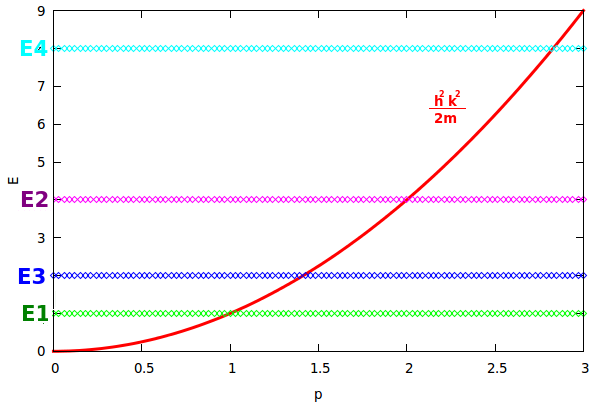
\includegraphics[scale=0.5]{obrazki/wykl_7_obrazek3.png}\end{center}
\subsubsection{Rozkład Fermiego-Diraca}
\begin{enumerate}
\item Tw. Dla niezerowej temperatury średnia liczba fermionów przypadających na 1 stan jest określony rozkładem Fermiego-Diraca:
\begin{equation} f_{FD}(\Ep)=f_{FD}(\p)=\frac{1}{1+e^{\frac{\Ep-\mu}{k_BT}}}\end{equation}
\item Asymptotyczne zachowanie:\\
1) W niskich temperaturach:
\begin{equation}\lim\limits_{T \to 0}f_{FD}(\Ep)=\theta(\Ep-\mu)= \begin{cases} 1~~\text{dla}~\Ep < \mu \\ 0~~\text{dla}~\Ep >\mu\end{cases}\end{equation}
gdzie $\theta$ to funkcja schodkowa Heavi-Side'a.\\
2) W wysokich temperaturach rzędu $|E-\mu|>>k_BT$:
\begin{equation}\lim\limits_{\frac{|E-\mu|}{k_BT}\rightarrow\infty} f_{FD}(\Ep)=e^{-\frac{\Ep-\mu}{k_BT}}=f_B(\Ep)\end{equation}
gdzie $f_B$ to rozkład Boltzmanna.\\
3) W punkcie $\Ep=\mu$:
\begin{equation}f_{FD}(\Ep=\mu)=\frac{1}{1+1}=\frac{1}{2}\end{equation}
\item Jak wyznaczyć potencjał chemiczny $\mu$?\\
a) Z równania:
\begin{equation} N=(2\sigma+1)\sum_{\p}f_{FD}(\Ep)\end{equation}
W ośrodku nieskończonym:
\begin{equation}V\rightarrow\infty:~~N=(2\sigma+1)\frac{V}{(2\pi\hbar)^3}\int d^3p f_{FD}(\Ep)\end{equation}
b) z równania na koncentrację\\
Pamiętamy, że koncentracja elektronów to:
\begin{equation}n=\frac{N}{V}\end{equation}
gdzie V to objętość naczynia, w którym są elektrony.\\
Zatem:
\begin{equation}n=N=\frac{2\sigma+1}{(2\pi\hbar)^3}\int d^3p f_{FD}(\Ep)=\frac{2\sigma+1}{(2\pi\hbar)^3}\int d^3p \frac{1}{1+e^{\frac{\frac{p^2}{2m}-\mu}{k_BT}}}\end{equation}
n można fizycznie zmierzyć w pomiarze efektu Halla.
\item Ogólny kształt funkcji rozkładu Fermiego-Diraca:
\begin{center}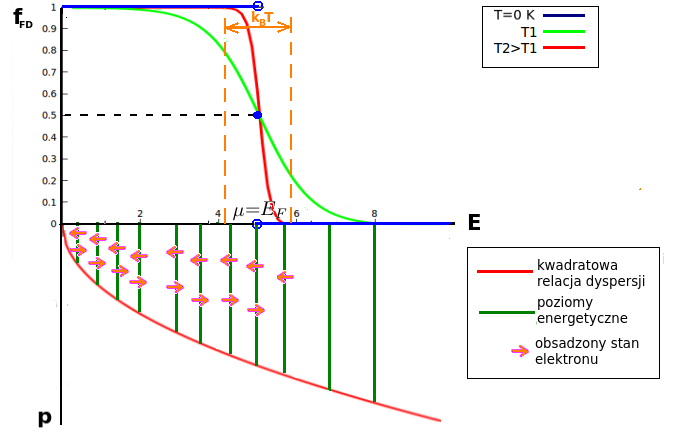
\includegraphics[scale=0.75]{obrazki/wykl_7_obrazek4.png}\end{center}
Zgodnie z zakazem Pauliego, na każdym poziomie energetycznym są maksymalnie 2 elektrony- o przeciwnych spinach.\\
Elektrony mogą przeskakiwać ze stanów obsadzonych do stanów nieobsadzonych w  okolicy Energii Fermiego, w przedziale o szerokości $k_BT$.
\item Pochodna funkcji rozkładu Fermiego Diraca:\\
W $T=0 K$:
\begin{equation}\frac{\partial f_{FD}(\Ep)}{\partial E}=-\delta(\Ep-E_F)\end{equation}
W $T>0 K$:
\begin{equation}\frac{\partial f_{FD}(\Ep)}{\partial E}=-\frac{1}{\pi}\frac{k_BT}{(\Ep-E_F)^2+(k_BT)^2}\end{equation}
Powyższy wyraz to Lorencjan. \\
Jest to tzw. funkcja spektralna.[NO I??????????????????? CO TO JEST??]
\begin{center}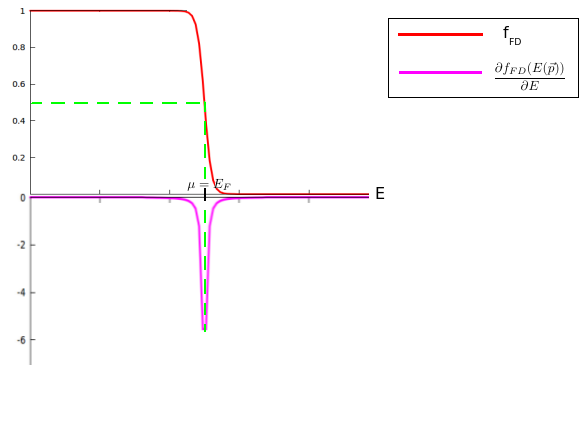
\includegraphics[scale=0.5]{obrazki/wykl_7_obrazek5.png}\end{center}
\end{enumerate}
\subsection{Całki zdarzeń $I[\f]$- przybliżenie czasu relaksacji (PCR)}
\subsubsection{Całka zdarzeń- definicja}
Uw. Aby uzyskać czytelność wzorów, dalej w indeksach pominięto wektor nad pędami: $\p\equiv p$.
\begin{equation}I[\f]=\sum_{p'}\{S_{p'p}-S_{pp'}\}\end{equation}
gdzie $\p'$ to pęd końcowy, natomiast:
\begin{equation}S_{pp'}=Q_{pp'}\f[1-\fp]\end{equation}
gdzie:\\
\begin{itemize}
\item Q opisuje szybkość przejść między $\p$ i $\p'$ (czyli szybkość rozproszeń);
\item$\f$ to stan, w którym jest elektron;
\item$\fp$ to stan, do którego elektron się rozprasza (na atomie).
\item$\r$ w obu wyrazach jest ten sam, czyli elektron rozprasza się w 1 punkcie przestrzeni (nie przemieszcza się w czasie rozproszenia).
\begin{center}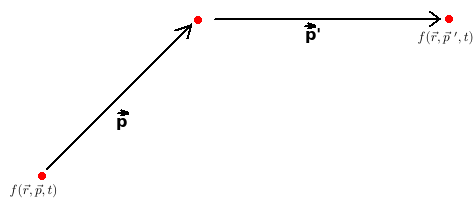
\includegraphics[scale=0.5]{obrazki/wykl_7_obrazek6.png}\end{center}
\end{itemize}
\subsubsection{Równanie Boltzmana- rozwiązanie}
\begin{enumerate}
\item Ogólna postać, z zastosowaniem definicji całki zdarzeń:
\begin{equation}\partial_t\f+\v\cdot\nab{r}\f+q(E+\v\times\B)\cdot\nabla_p\f=\end{equation}
\begin{equation} =\sum_{p'}\{Q_{p'p}\fp(1-\f)-Q_{pp'}\f(1-\fp\}\nonumber\end{equation}
\item Zasada równowagi mikroskopowej:\\
Szybkość przejścia ze stanu 1 do stanu 2 i szybkość przejścia ze stanu 2 do stanu 1 jest taka sama:
\begin{equation}Q_{p'p}=Q_{pp'}\end{equation}
\item Zatem całka zdarzeń:
\begin{equation}I[\f]=\sum_{p'}Q_{p'p}\{\fp-\fp\f-\f+\f\fp\}=\end{equation}
\begin{equation}=\sum_{p'}Q_{p'p}\{\fp-\f\}=\nonumber\end{equation}
\begin{equation}=-\f\sum_{p'}Q_{p'p}\{1-\frac{\fp}{\f}\}\nonumber\end{equation}
\item Wprowadzenie czasu relaksacji:\\
Wymiarem sumy obecnej w całce zdarzeń jest wymiar szybkości $Q_{p'p}$, czyli $\frac{1}{s}$. To jest przesłanka, by traktować tę sumę jako \textbf{odwrotność czasu relaksacji} $\tau$:
\begin{equation}\sum_{p'}Q_{p'p}\{1-\frac{\fp}{\f}\}\equiv=\tau^{-1}(\r,\p,t)\end{equation}
zatem: 
\begin{equation}I[\f]=-\frac{\f}{\tau(\r,\p,t)}\end{equation}
Wówczas równanie Boltzmana:
\begin{equation}\partial_t\f+\v\cdot\nab{r}\f+\underbrace{q(E+\v\times\B)}_{\text{siła Lorentza}~F_L}\cdot\nabla_p\f=-\frac{\f}{\tau(\r,\p,t)}\end{equation}
Wprowadza się również wyrażenie:
\begin{equation}\tau^{-1}(\p)=\sum_{p'}Q_{pp'}\end{equation}
które jest miarą siły oddziaływania z atomami (rozpraszania na nich).
Wówczas:
\begin{equation}I[\f]=\frac{\f}{\tau(\p)}-\sum_{p'}Q_{p'p}\fp=\end{equation}
\begin{equation}=\frac{\f-\frac{\sum_{p'}Q_{p'p}\fp}{\sum_{p'}Q_{p'p}}}{\tau(\p)}=\nonumber\end{equation}
\begin{equation}=\frac{\f-f_0(\r,\p,t)}{\tau(\p)}\nonumber\end{equation}
gdzie:
\begin{itemize}
\item $\f$ to nierównowagowa funkcja rozkładu
\item $f_0(\r,\p,t)$ to równowagowa funkcja rozkładu\\
\end{itemize}
Dla gazu elektronowego:
\begin{equation}f_0(\r,\p,t)=f_{FD}\end{equation}

\item Równanie Boltzmana zyskuje postać:
\begin{equation}\partial_t\f+\v\cdot\nab{r}\f+\vec{F}_L\cdot\nabla_p\f=-\frac{\f-f_0(\r,\p,t)}{\tau(\p)}\end{equation}
\item Założenia\\
\begin{itemize}
\item[I.] Badamy układy stacjonarne: $\f=f(\r,\p)$ - nie zależy od $t$
\item[II.] Układ jest jednorodny: $f(\r,\p)=f(\p)$ - nie zależy od $\r$
\end{itemize}
Założenia te wprowadzają idealny gaz elektronowy.
\item Zatem równanie Boltzmanna dla idealnego gazu elektronowego:
\begin{equation}q\E\cdot\nabla_{p}f(\p)=-\frac{f(\p)-f_0(\p)}{\tau(\p)}~~~~/\cdot\tau(\p)\end{equation}
Biorąc pod uwagę, że $q=-e$:
\begin{equation}e\tau(\p)\E\cdot\nabla_{p}f(\p)=f(\p)-f_0(\p)\end{equation}
Stąd:
\begin{equation}\underbrace{f(\p)}_{\text{funkcja nierównowagowa}} =\underbrace{f_0(\p)}_{\text{funkcja równowagowa}} +\underbrace{e\tau(\p)E\cdot\nabla_{p}f(\p)}_{\delta f}\label{f.nierownowagowa}\end{equation}
gdzie:\\
$\delta f$ to odchylenie od stanu równowagowego (bo $\nabla_{p}f$). Zakładamy, że zaburzenie to jest niewielkie:
\begin{equation}f_0(\p)>>\delta f(\p)\end{equation}
Powyższe równanie ma postać rozwinięcia w szereg Taylora do 1. wyrazu
\item Wniosek:\\
Jeśli przyłożymy małe pole $\E$, to obowiązuje przybliżenie czasu urojonego i funkcję rozkładu rozwija się w szereg Taylora do 1. wyrazu (bo wychylenie jest niewielkie).\\
\item Iteracyjne rozwiązywanie równania (\ref{f.nierownowagowa}):
\begin{equation}f_1(\p)=f_0(\p)+e\tau(\p)\E\cdot\nabla_{p}f_0(\p)
\simeq
f_0(\p+\underbrace{e\tau(\p)}_{\delta \p}\E) \end{equation}
Wniosek:
Zmiana pędu spowodowana włączeniem pola $\E$ przesuwa rozkład $f_{FD}$ o pewne $\delta p$:
\begin{center}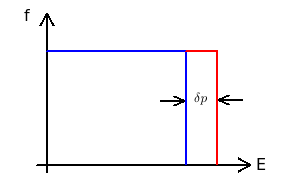
\includegraphics[scale=0.75]{obrazki/wykl_7_obrazek7.png}\end{center}
W książkach ta sama relacja jest pokazywana często w następujący sposób:
\begin{center}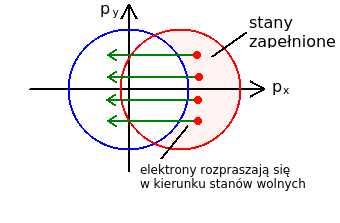
\includegraphics[scale=1]{obrazki/wykl_7_obrazek8.png}\end{center}
\item Gęstość prądu
Pamiętamy:
\begin{equation}\j=\sigma\E\end{equation}
Teraz możemy obliczyć:
\begin{equation}\j=evn=\frac{e}{(2\pi\hbar)^3}\int d^3p\v(\p)f(\p)=\end{equation}
\begin{equation}=\frac{e}{(2\pi\hbar)^3}\int d^3p\v(\p)\{f_0(\p)+e\tau(\p)\E\cdot\nabla_{p}f(\p)\}\nonumber\end{equation}
Funkcja równowagowa:
\begin{equation}f_0\propto p^2\end{equation}
opisuje pasma niebiorące udział w transporcie, zatem:
\begin{equation}\int d^3p\v f_0(\p)=0\end{equation}
Zatem:
\begin{equation}\j=\frac{e^2}{(2\pi\hbar)^3} \int d^3p\v(\p)\tau(\p)\nabla_{p}f(\p)\cdot\E\end{equation}
Ale:
\begin{equation} \nabla_p f(\p)=\frac{\partial E(\p)}{\partial p}\frac{\partial f(\Ep)}{\partial E}=\frac{\p}{m}\frac{\partial f}{\partial E}=\v \frac{\partial f}{\partial E}\end{equation}
Zatem: 
\begin{equation}\j=\underbrace{\frac{e^2}{(2\pi\hbar)^3} \int d^3p [\v(\p)\otimes\v(\p)]\tau(\p)\frac{\partial f}{\partial E}}_{\sigma}\E\end{equation}
\end{enumerate}





\end{document}


